\documentclass[11pt,a4paper]{article}

% --- Encoding & Sprache ---
\usepackage[T1]{fontenc}
\usepackage[utf8]{inputenc}
\usepackage[ngerman]{babel}

% --- Layout & Typografie ---
\usepackage[a4paper,margin=1.5cm]{geometry} % Schmaler Rand
\usepackage{setspace}
\usepackage{enumitem}
\usepackage{hyperref}
\usepackage{graphicx}
% Legt Suchpfade für Bilder fest (damit Bilddateien im lokalen Verzeichnis sowie im Unterordner "images" gefunden werden)
\graphicspath{{.}{./images/}}
\usepackage{array}
\usepackage{booktabs}
\usepackage{fancyhdr}
\usepackage{xcolor}
\usepackage{csquotes}

% --- Hyperref Setup ---
\hypersetup{
  pdftitle={HopIn Temporäre Event-Gruppen (HCD A5A)},
  pdfauthor={Kevin Forter, Benjamin Feichtlbauer},
  pdfsubject={Prototyp-Dokumentation},
  pdfkeywords={HCD, Prototyp, Event-Organisation, temporäre Gruppen},
  colorlinks=true,
  linkcolor=black,
  urlcolor=blue,
  citecolor=black
}

% --- Header / Footer ---
\usepackage{fancyhdr}
\pagestyle{fancy}
\fancyhf{}
\fancyhead[L]{Bachelor Informatik}
\fancyhead[C]{Human Centered Design}
\fancyhead[R]{Aufgabe~5}
\fancyfoot[C]{Feichtlbauer, Forter\,–\,Seite~\thepage}
\setlength{\headheight}{15pt}


% --- Absätze & Listen ---
\setlength{\parskip}{6pt}
\setlength{\parindent}{0pt}
\setlist[itemize]{leftmargin=1.2em}
\setlist[enumerate]{leftmargin=1.4em}

% --- Nützliche Makros ---
\newcommand{\appname}{\textbf{HopIn}}

\begin{document}

% --- Titelseite ---
\begin{titlepage}
  \centering
  \vspace*{2cm}
  {\Huge Prototyping – HCD Aufgabe 5\par}
  \vspace{0.8cm}
  {\Large Prototyping Report\par}
  \vspace{2.0cm}
  {\large Benjamin~Feichtlbauer\\Kevin~Forter\par}
  {\large Bachelor Informatik / Computer Science\par}
  {\large Lehrveranstaltung: Human Centered Design\par}
  {\large \today\par}
\end{titlepage}


\section*{Projektidee}
\appname{} ist eine mobile App (bzw.\ Web-App), mit der Nutzer temporäre Gruppen für Events erstellen können, zum Beispiel für Partys, Ausflüge, Sporttreffen oder Uni-Projekte.
Im Gegensatz zu klassischen Messenger-Gruppen wie WhatsApp, die nach dem Event bestehen bleiben, werden Gruppen bei \appname{} automatisch archiviert, sobald das Event endet.
So bleibt der Kommunikationsbereich aufgeräumt, übersichtlich und fokussiert auf das Wesentliche: gemeinsam planen, durchführen und abschließen.

\section*{Zielsetzung}
Das Ziel von \appname{} ist es, die kurzfristige Event-Organisation zu vereinfachen und gleichzeitig digitale Ordnung zu fördern.
Nutzer sollen schnell Gruppen erstellen, andere einfach einladen (per Link oder QR-Code) und alle relevanten Informationen wie Chat, To-Dos und Umfragen an einem Ort bündeln können.
Nach Ende des Events verschwindet die Gruppe automatisch aus der aktiven Ansicht, bleibt aber im Archiv zur Einsicht erhalten.

\section*{Zielgruppe und Ziele des Prototyps (Use Cases)}
\textbf{Zielgruppe:} Personen, die häufig spontane oder kurzfristig planbare Anlässe organisieren (Studierende, Berufstätige, Elternvertretungen) und dabei klare, temporäre Kommunikationsräume bevorzugen.

\textbf{Ziele des Prototyps:}
\begin{itemize}
  \item Schnelle Erstellung temporärer Event-Gruppen mit Titel, Datum/Uhrzeit und optionalen Rollen.
  \item Reibungsloses Einladen via Link oder QR-Code ohne Nummernspeicherung.
  \item Bündelung relevanter Funktionen: Chat, To-Dos (wer bringt was?), Umfragen (Termin/Ort) und Dateien.
  \item Automatisches Archivieren der Gruppe nach Event-Ende, weiterhin lesender Zugriff im Archiv.
  \item Übersicht über bevorstehende, laufende und archivierte Events.
\end{itemize}

\section*{Persona 1: Lisa Sommer (21) Studentin}
\textbf{Beschreibung:} Lisa studiert Medienwissenschaften, wohnt in einer WG und organisiert oft spontane WG-Partys oder kleine Geburtstagsrunden. Sie hasst es, ständig neue WhatsApp-Gruppen zu erstellen, die danach nie wieder genutzt werden.

\textbf{Ziele:}
\begin{itemize}
  \item Events unkompliziert planen
  \item Leute einfach einladen (ohne Nummern zu speichern)
  \item Ordnung in ihren Kommunikations-Apps behalten
\end{itemize}

\textbf{Pain Points:}
\begin{itemize}
  \item Unübersichtliche WhatsApp-Gruppen
  \item Alte Gruppen bleiben bestehen
  \item Planungstools sind oft zu kompliziert
\end{itemize}

\textbf{User Story:}
\begin{quote}
Als Studentin möchte ich für meine WG-Party schnell eine temporäre Gruppe erstellen können, damit ich alle Gäste koordinieren kann und die Gruppe sich nach der Party automatisch archiviert, damit mein Chat wieder sauber bleibt.
\end{quote}

\section*{Persona 2: Jonas Keller (28) Berufstätiger}
\textbf{Beschreibung:} Jonas ist Softwareentwickler und organisiert regelmäßig Wochenend-Aktivitäten mit Freunden, zum Beispiel Fußballspiele oder Grillabende. Er möchte die Organisation schlank und effizient halten, ohne dauerhafte Gruppen oder zu viel Chat-Spam.

\textbf{Ziele:}
\begin{itemize}
  \item Spontane Gruppen einfach erstellen
  \item Übersicht über bevorstehende Events
  \item Klare Trennung zwischen Arbeit und Freizeit
\end{itemize}

\textbf{Pain Points:}
\begin{itemize}
  \item Zu viele aktive Gruppenchats
  \item Schwer, alles im Blick zu behalten
  \item Kein einfaches Tool für kurzfristige Planung
\end{itemize}

\textbf{User Story:}
\begin{quote}
Als Berufstätiger möchte ich temporäre Gruppen für Freizeitaktivitäten erstellen können, um Termine und Aufgaben (zum Beispiel wer bringt was mit?) zu organisieren und danach automatisch alles ins Archiv verschieben lassen, damit ich nicht alles manuell löschen muss.
\end{quote}

\section*{Persona 3: Sarah Baumann (35) Mutter und Elternbeirätin}
\textbf{Beschreibung:} Sarah koordiniert Schulaktivitäten, Ausflüge und Elternabende. Sie nutzt WhatsApp-Gruppen, aber es wird schnell chaotisch, wenn für jedes Event eine neue Gruppe bleibt.

\textbf{Ziele:}
\begin{itemize}
  \item Übersicht über vergangene und kommende Schul-Events
  \item Einfache Kommunikation mit anderen Eltern
  \item Strukturiertes Planen ohne Informationsverlust
\end{itemize}

\textbf{Pain Points:}
\begin{itemize}
  \item Alte Gruppen bleiben bestehen
  \item Teilnehmer vergessen, Gruppen zu verlassen
  \item Zu viele Chats ohne klare Struktur
\end{itemize}

\textbf{User Story:}
\begin{quote}
Als Elternbeirätin möchte ich für jedes Schulfest eine temporäre Gruppe erstellen können, damit ich Einladungen, Aufgaben und Infos teilen kann und nach dem Event die Gruppe automatisch archiviert wird, um Ordnung zu behalten.
\end{quote}

\section*{Dokumentation des Prototyps}

Dieser Abschnitt beschreibt den interaktiven Prototyp, die exemplarischen Anwendungsszenarien sowie die zentralen Bildschirme. Die Abbildungen stammen aus dem Figma‑Prototyp und befinden sich im gleichen Ordner wie diese Datei.

\subsection*{Use Cases und Navigationsfluss}
Der Prototyp unterstützt drei wesentliche Nutzungsfälle:
\begin{itemize}
  \item \textbf{UC1 – Event anlegen:} Über den Profil‑Screen kann ein neues Event mit Name, Ort, Beginn und Ende erstellt werden (Abb.~\ref{fig:create}). Nach dem Speichern erscheint das Event in der Übersicht und ist für eingeladene Personen sichtbar.
  \item \textbf{UC2 – Gäste einladen:} Im Event‑Detail lässt sich über den Share‑Button ein QR‑Code sowie ein sechsstelliger Zahlencode generieren (Abb.~\ref{fig:share}). Gäste können so dem Event beitreten, ohne ihre Kontaktdaten freizugeben.
  \item \textbf{UC3 – Medien sammeln und archivieren:} Während der Veranstaltung können Fotos im Album (Abb.~\ref{fig:album}) geteilt werden. Nach Ablauf des Events wird es automatisch in die Archiv‑Ansicht verschoben (Abb.~\ref{fig:archive}) und bleibt dort lesbar.
\end{itemize}

Der Navigationsfluss ist bewusst einfach gehalten: Nach dem \textbf{Login} (Abb.~\ref{fig:login}) landet der Nutzer auf der \textbf{Home}‑Seite (Abb.~\ref{fig:home}) mit einer Liste aller bevorstehenden Veranstaltungen. Eine Tab‑Bar ermöglicht jederzeit den Wechsel zum \emph{Archive} (Abb.~\ref{fig:archive}) oder zum \emph{Profile} (Abb.~\ref{fig:profile}). Ein Tap auf eine Event‑Karte in der Home‑Ansicht öffnet das \textbf{Event‑Detail} (Abb.~\ref{fig:eventinfo}); von dort führen Buttons zum Einladen (QR‑Ticket) und zum Album. Neue Events werden über den Profil‑Screen angelegt.

\subsection*{Bildschirmübersicht}

\paragraph{Login / Sign‑Up}\mbox{}\\
Der Einstiegspunkt für alle Nutzer (Abb.~\ref{fig:login}): Neben E‑Mail/Passwort‑Felder gibt es Social‑Login‑Optionen. Ein freundlicher Begrüßungstext motiviert zur Nutzung der App.

\paragraph{Home / Upcoming Events}\mbox{}\\
Diese Startseite (Abb.~\ref{fig:home}) listet alle bevorstehenden Events. Das nächste Event wird farbig hervorgehoben und zeigt Titel, Ort, Countdown sowie kleine Avatare der bereits zugesagten Gäste. Weitere Events erscheinen als Karten darunter mit Datum, Ort und Organisator.

\paragraph{Archive}\mbox{}\\
In der Archiv‑Ansicht (Abb.~\ref{fig:archive}) werden vergangene Veranstaltungen nach Jahren gruppiert dargestellt. So können Nutzer vergangene Events noch einmal durchsehen, ohne ihre aktuelle Übersicht zu verlieren.

\paragraph{Profil}\mbox{}\\
Der Profil‑Screen (Abb.~\ref{fig:profile}) zeigt den Avatar, den Namen und den Benutzernamen des Nutzers. Zwei interaktive Bereiche erlauben das Anlegen eines neuen Events (\emph{Create Event}) sowie den Zugriff auf eigene Veranstaltungen (\emph{Your Events}).

\paragraph{Event‑Detail}\mbox{}\\
In der Detailansicht (Abb.~\ref{fig:eventinfo}) werden das Titelbild, der Name, der Ort, das Datum und der Veranstalter des Events präsentiert. Die Gästeliste wird durch farbcodierte Buttons dargestellt, die zwischen offenen Einladungen, Absagen und Zusagen unterscheiden. Unterhalb befindet sich eine Bildvorschau und ein Button zum Öffnen des Albums. Der Share‑Button generiert ein QR‑Ticket zum Einladen.

\paragraph{QR‑Einladung}\mbox{}\\
Das Share‑Overlay (Abb.~\ref{fig:share}) erinnert an eine Eintrittskarte: Es zeigt einen QR‑Code und einen Zahlencode. Start- und Endzeit des Events werden ebenfalls angezeigt, sodass Gäste den Kontext kennen.

\paragraph{Album}\mbox{}\\
In der Album‑Ansicht (Abb.~\ref{fig:album}) können alle während eines Events geteilten Bilder in einem Raster angesehen werden. Nutzerinnen und Nutzer können durch die Bilder scrollen und neue Fotos hinzufügen.

\paragraph{Event anlegen}\mbox{}\\
Über die Eingabemaske \emph{Create Event} (Abb.~\ref{fig:create}) werden Name und Ort des Events sowie Start- und Endzeit definiert. Eine Umschaltoption aktiviert bei Bedarf die Chat‑Funktion. Nach Bestätigung erscheint das Event in der Home‑Ansicht.

\subsection*{Abbildungen}

\begin{figure}[h]
  \centering
  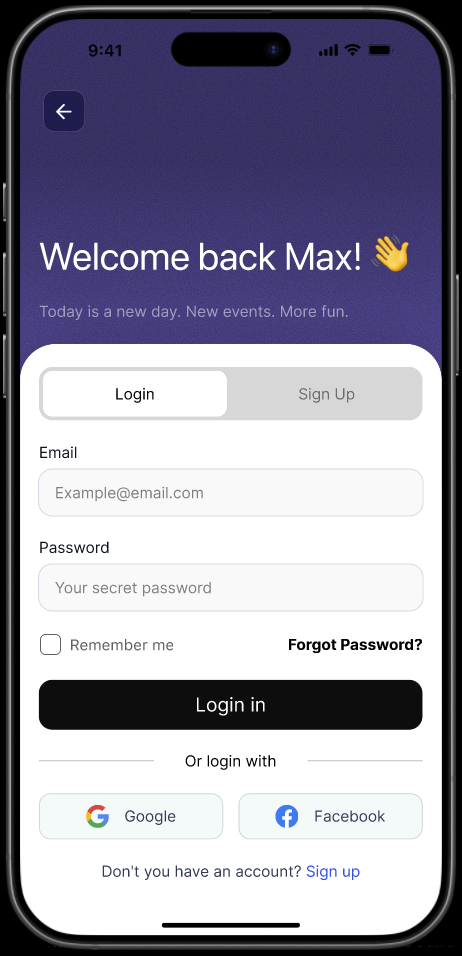
\includegraphics[width=0.6\textwidth]{image-2.png}
  \caption{Login‑ und Sign‑Up‑Screen mit E‑Mail/Passwort‑Eingabe sowie Social‑Login‑Optionen.}
  \label{fig:login}
\end{figure}

\begin{figure}[h]
  \centering
  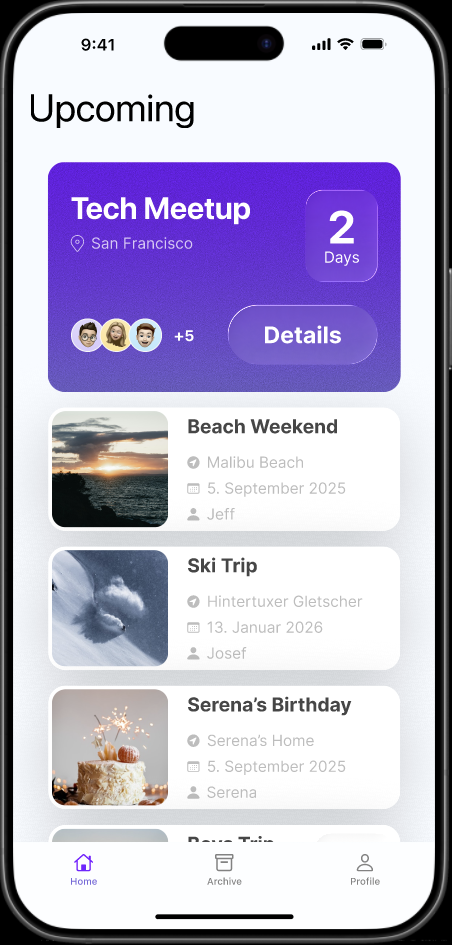
\includegraphics[width=0.6\textwidth]{image-3.png}
  \caption{Home‑Ansicht: anstehende Events mit hervorgehobener nächster Veranstaltung und weiteren Karten.}
  \label{fig:home}
\end{figure}

\begin{figure}[h]
  \centering
  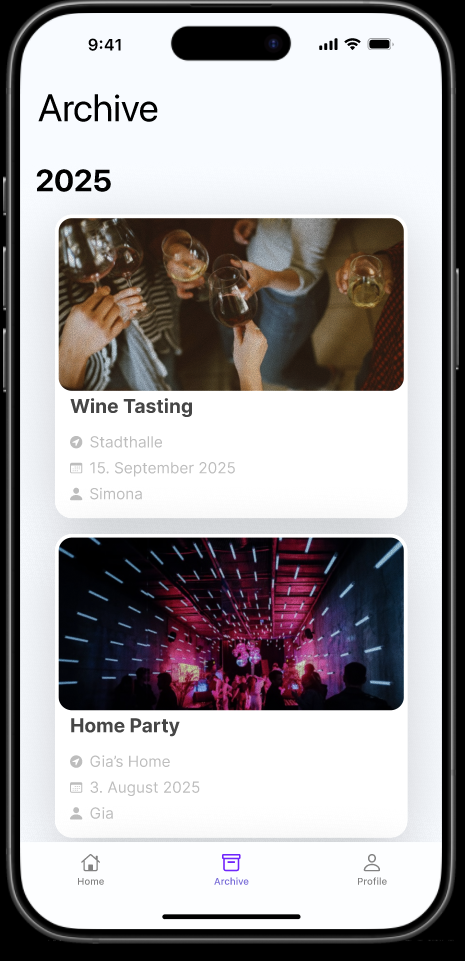
\includegraphics[width=0.6\textwidth]{image-4.png}
  \caption{Archiv‑Ansicht: vergangene Veranstaltungen gruppiert nach Jahr.}
  \label{fig:archive}
\end{figure}

\begin{figure}[h]
  \centering
  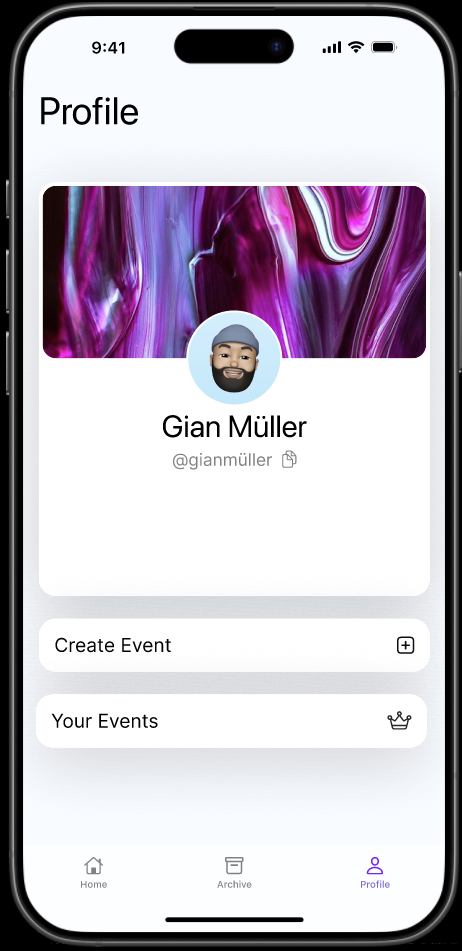
\includegraphics[width=0.6\textwidth]{image-5.png}
  \caption{Profil‑Screen: Avatar, Name, Benutzername sowie Optionen zum Erstellen und Verwalten eigener Events.}
  \label{fig:profile}
\end{figure}

\begin{figure}[h]
  \centering
  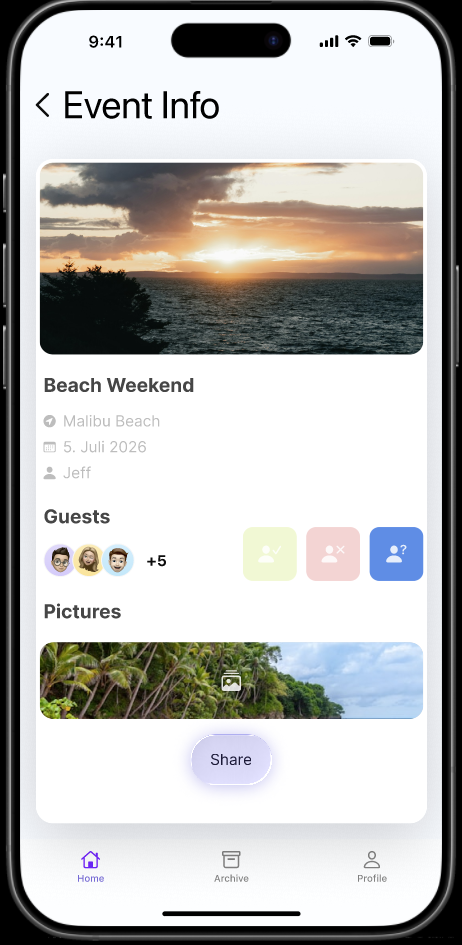
\includegraphics[width=0.6\textwidth]{image-6.png}
  \caption{Event‑Detail: Titelbild, Eckdaten, Gästeliste und Vorschau des Albums. Über den \emph{Share}-Button lässt sich ein QR‑Ticket erzeugen.}
  \label{fig:eventinfo}
\end{figure}

\begin{figure}[h]
  \centering
  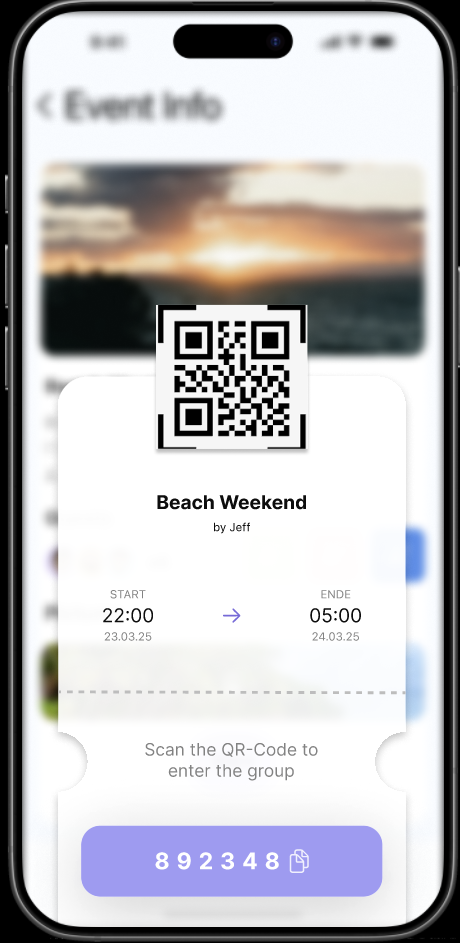
\includegraphics[width=0.6\textwidth]{image-7.png}
  \caption{QR‑Einladung: Ticket mit QR‑Code und Zahlencode für den schnellen Beitritt zum Event.}
  \label{fig:share}
\end{figure}

\begin{figure}[h]
  \centering
  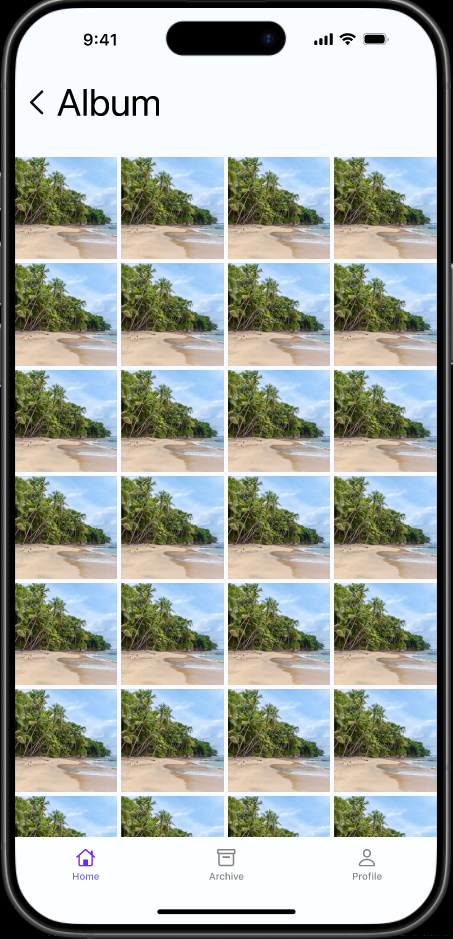
\includegraphics[width=0.6\textwidth]{image-8.png}
  \caption{Album‑Ansicht: Rasterdarstellung der während des Events geteilten Bilder.}
  \label{fig:album}
\end{figure}

\begin{figure}[h]
  \centering
  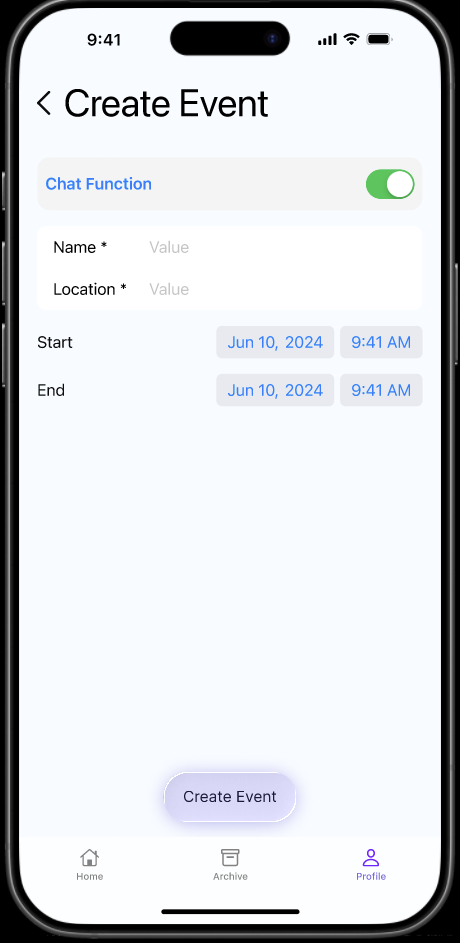
\includegraphics[width=0.6\textwidth]{image-9.png}
  \caption{Formular zur Event‑Erstellung: Eingabefelder für Name, Ort, Start- und Endzeit sowie Umschalter für die Chat‑Funktion.}
  \label{fig:create}
\end{figure}

\subsection*{Link (mit Bearbeitungszugriff)}
\textbf{Prototyp‑URL:} \url{https://www.figma.com/file/Dmgm18zgv7DBHrGzGCSv53?node-id=3:3&locale=de&type=design}
\end{document}